\section{\img{figs/RelBench_favicon.png}~\BenchmarkName: A Benchmark for \AreaName}\label{sec: benchmark}
\begin{figure}[h]
    \centering
    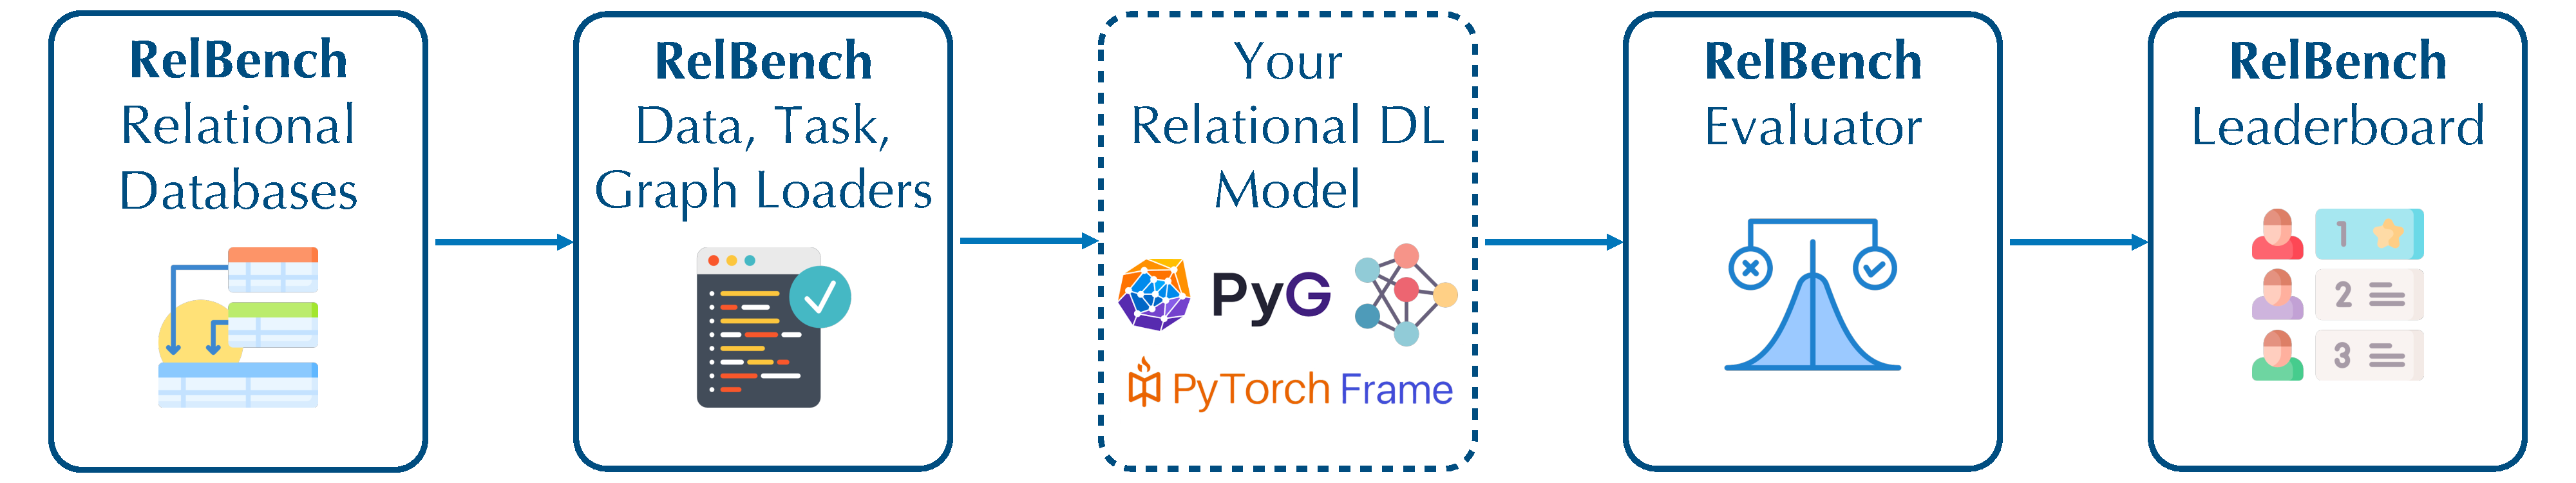
\includegraphics[width=\textwidth]{figs/relbench-fig.pdf}
    \caption{\textbf{Overview of \BenchmarkName.} \BenchmarkName enables training and evaluation of machine learning models on relational data. \BenchmarkName supports deep learning framework agnostic data loading, task specification, standardized data splitting, and transforming data into graph format. \BenchmarkName provides standardized evaluation metric computations, and a leaderboard for tracking progress.  We additionally provide example training scripts built using PyTorch Geometric and PyTorch Frame.}
    \label{fig:rtb-fig}
\end{figure}

We introduce \BenchmarkName, an open benchmark for \AreaName. The goal of \BenchmarkName is to facilitate scalable, robust, and reproducible machine learning research on relational tables. \BenchmarkName curates a diverse set of large-scale, challenging, and realistic benchmark databases and defines meaningful predictive tasks over these databases. In addition, \BenchmarkName develops a Python library for loading relational tables and tasks, constructing data graphs, and providing unified evaluation for predictive tasks. It also integrates seamlessly with existing Pytorch Geometric and PyTorch Frame functionalities. In its beta release\footnote{Website: \url{https://relbench.stanford.edu}}\footnote{Package: \url{https://github.com/snap-stanford/relbench}}, we announce the first two real-world relational databases, each with two curated predictive tasks. 

In the subsequent sections (Sec.~\ref{sec:amazon} and~\ref{sec:stack}), we describe in detail the two relational databases and the predictive tasks. For each database, we show its entity relational diagrams and important statistics. For each task, we define the task formulation, entity filtering, significance of the task, and also unified evaluation metric. Finally, we demonstrate the usage of the \BenchmarkName's package in Sec.~\ref{sec:package}.

\subsection{\BenchmarkName Package}\label{sec:package}

The \BenchmarkName package is designed to allow easy and standardized access to \AreaName for researchers to push the state-of-the-art of this emerging field. It provides Python APIs to (1) download and process relational databases and their predictive tasks; (2) load standardized data splits and generate relevant train/validation/test tables; (3) evaluate on machine learning predictions. It also provides a flexible ecosystems of supporting tools such as automatic conversion to PyTorch Geometric graphs and integration with Pytorch Frame to produce embeddings for diverse column types. We additionally provide end-to-end scripts for training using \BenchmarkName package with GNNs and XGBoost~\citep{chen2016xgboost}. We refer the readers to the code repository for a more detailed understanding of \BenchmarkName. Here we demonstrate the core functionality. 


To load a relational database, simply do:

\vspace{-3mm}
\begin{minted}[frame=lines,
framesep=2mm,
baselinestretch=1,
fontsize=\footnotesize
]{python}
from relbench.datasets import get_dataset
dataset = get_dataset(name="rel-amazon")
\end{minted}
\vspace{-3mm}

It will load the relational tables and process it into a standardized format. Next, to load the predictive task and the relevant training tables, do:

\vspace{-3mm}
\begin{minted}[frame=lines,
framesep=2mm,
baselinestretch=1,
fontsize=\footnotesize
]{python}
task = dataset.get_task("rel-amazon-ltv")
task.train_table, task.val_table, task.test_table # training/validation/testing tables
\end{minted}
\vspace{-3mm}

It automatically constructs the training table for the relevant predictive task. Next, after the user trains the machine learning model, the user can use \BenchmarkName standardized evaluator:
\vspace{-3mm}
\begin{minted}[frame=lines,
framesep=2mm,
baselinestretch=1,
fontsize=\footnotesize
]{python}
task.evaluate(pred)
\end{minted}
\vspace{-3mm}


\subsection{Temporal Splitting}

Every dataset in \BenchmarkName has a validation timestamp $t_{\text{val}}$ and a test timestamp $t_{\text{test}}$. These are shared for all tasks in the dataset.
The test table for any task comprises of labels computed for the time window from $t_{\text{test}}$ to $t_{\text{test}} + \delta$, where the window size $\delta$ is specified for each task. Thus the model must make predictions using only information available up to time $t_{\text{test}}$. Accordingly, to prevent accidental temporal leakage at test time \BenchmarkName only provides database rows with timestamps up to $t_{\text{test}}$ for training and validation purposes. \BenchmarkName also provides default train and validation tables. The default validation table is constructed similar to the test table, but with the time window being $t_{\text{val}}$ to $t_{\text{val}} + \delta$. To construct the default training table, we first sample time stamps $t_i$ starting from $t_{\text{val}} - \delta$ and moving backwards with a stride of $\delta$. This allows us to benefit from the latest available training information. Then for each $t_i$, we apply an entity filter to select the entities of interest (e.g., active users). Finally for each pair of timestamp and entity, we compute the training label based on the task definition. Users can explore other ways of constructing the training or validation table, for example by sampling timestamps with shorter strides to get more labels, as long as information after $t_{\text{val}}$ is not used for training.



\subsection{\Amazon: Amazon product review e-commerce database}\label{sec:amazon}


\begin{figure}[h] % 'h' for here
  \centering
  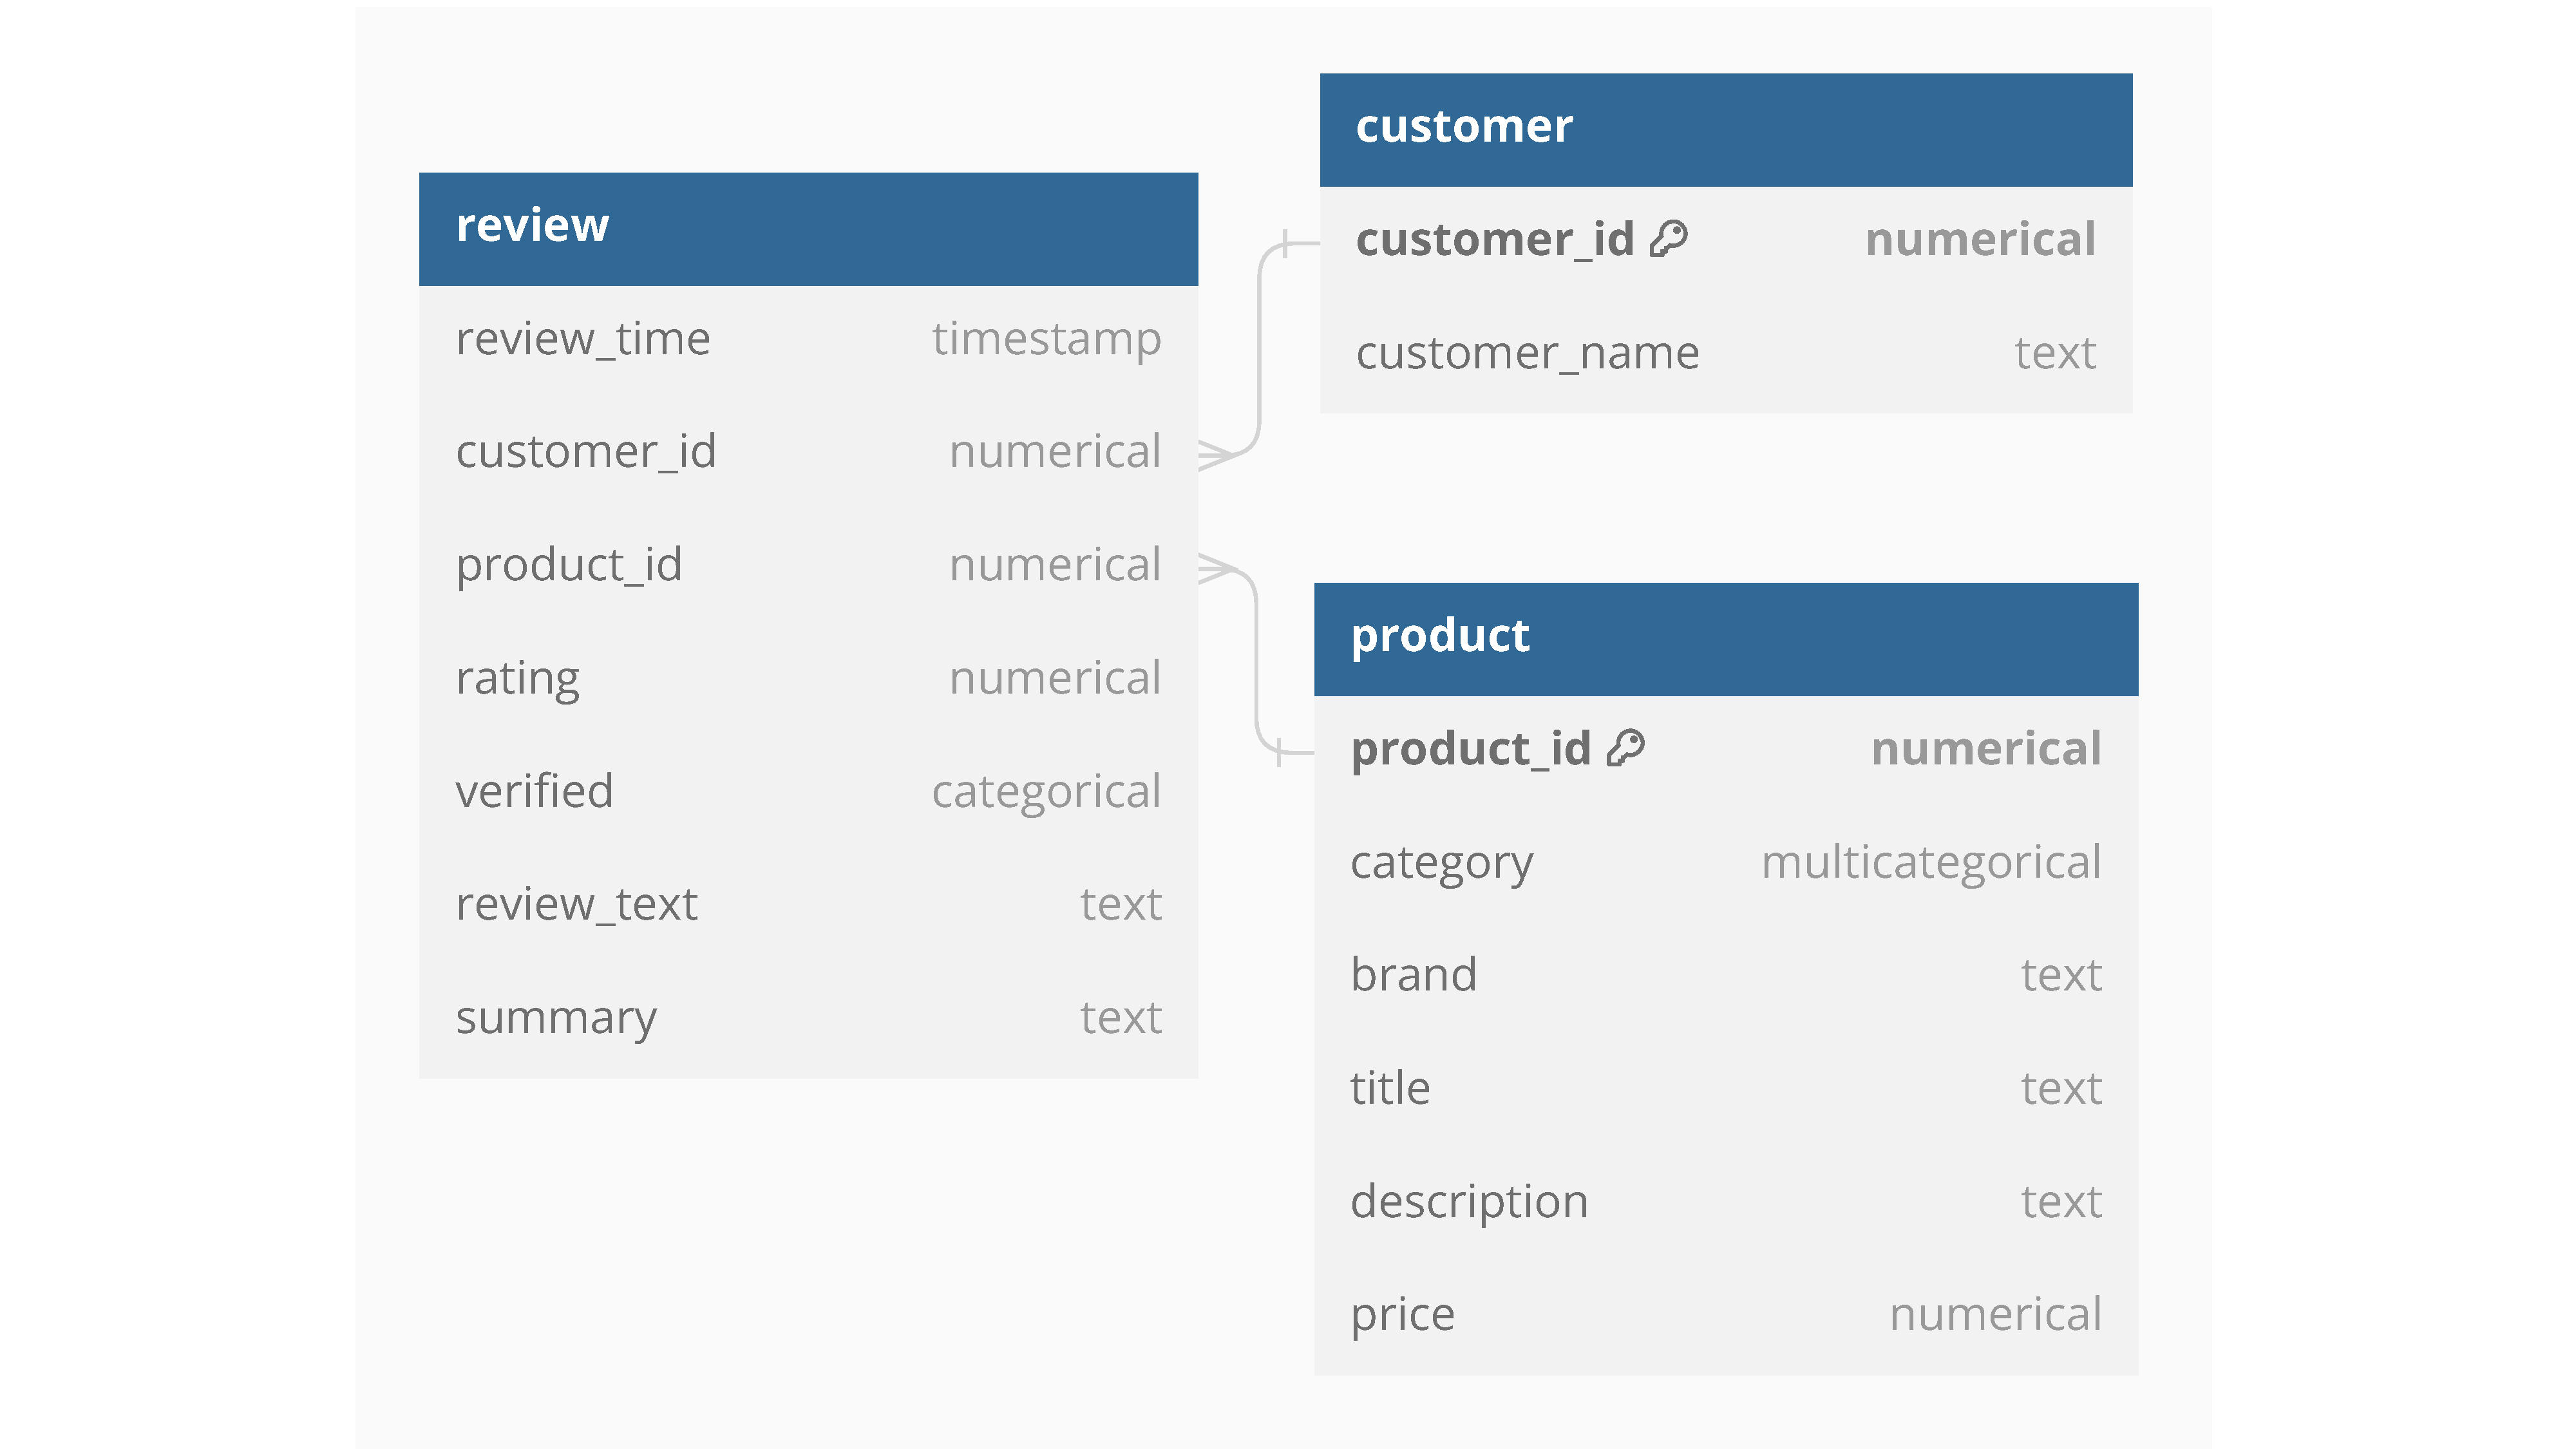
\includegraphics[width=0.5\linewidth]{figs/amazon-reviews.pdf}
  \caption{\Amazon contains two dimension tables (customers and products) and one fact table (reviews). Each review has a customer and a product foreign key. }
  
  \label{fig: product tables}
\end{figure}

\xhdr{Database overview} The \Amazon relational database stores product and user purchasing behavior across Amazon's e-commerce platform. Notably, it contains rich information about each product and transaction. The product table includes price and category information; the review table includes overall rating, whether the user has actually bought the product, and the text of the review itself. We use the subset of book-related products. The entity relationships are described in Fig. \ref{fig: product tables}.

\xhdr{Dataset statistics} \Amazon covers 3 relational tables and contains 1.85M customers, 21.9M reviews, 506K products. This relational database spans from 1996-06-25 to 2018-09-28. The validation timestamp $t_{\text{val}}$ is set to 2014-01-21 and the testing timestamp $t_{\text{test}}$ is 2016-01-01. Thus, tasks can have a window size up to 2 years.

\subsubsection{\AmazonLTV: Predict the life time value (LTV) of a user} 



\textbf{Task definition:} Predict the life time value of a user, defined as the sum of prices of the products that the user will buy and review in the next 2 years. 

\textbf{Entity filtering:} We filter on active users defined as users that wrote review in the past two years before the timestamp. 

\textbf{Task significance:} By accurately forecasting LTV, the e-commerce platform can gain insights into user purchasing patterns and preferences, which is essential when making strategic decisions related to marketing, product recommendations, and inventory management. Understanding a user's future purchasing behavior helps in tailoring personalized shopping experiences and optimizing product assortments, ultimately enhancing customer satisfaction and loyalty.

\textbf{Machine learning task:} Regression. The target ranges from \$0-\$33,858.4 in the given time window in the training table.


\textbf{Evaluation metric:} Mean Absolute Error (MAE).

\subsubsection{\AmazonChurn: Predict if the user churns} 

\textbf{Task definition:} Predict if the user will not buy any product in the next 2 years. 

\textbf{Entity filtering:} We filter on active users defined as users that wrote review in the past two years before the timestamp. 

\textbf{Task significance:} Predicting churn accurately allows companies to identify potential risks of customer attrition early on. By understanding which customers are at risk of disengagement, businesses can implement targeted interventions to improve customer retention. This may include personalized marketing, tailored offers, or enhanced customer service. Effective churn prediction enables businesses to maintain a stable customer base, ensuring sustained revenue streams and facilitating long-term planning and resource allocation.

\textbf{Machine learning task:} Binary classification. The label is 1 when user churns and 0 vice versus. 

\textbf{Evaluation metric:} Average precision (AP).


\subsection{\StackEx: Stack exchange question-and-answer website database}\label{sec:stack}

\begin{figure}[h] % 'h' for here
  \centering
  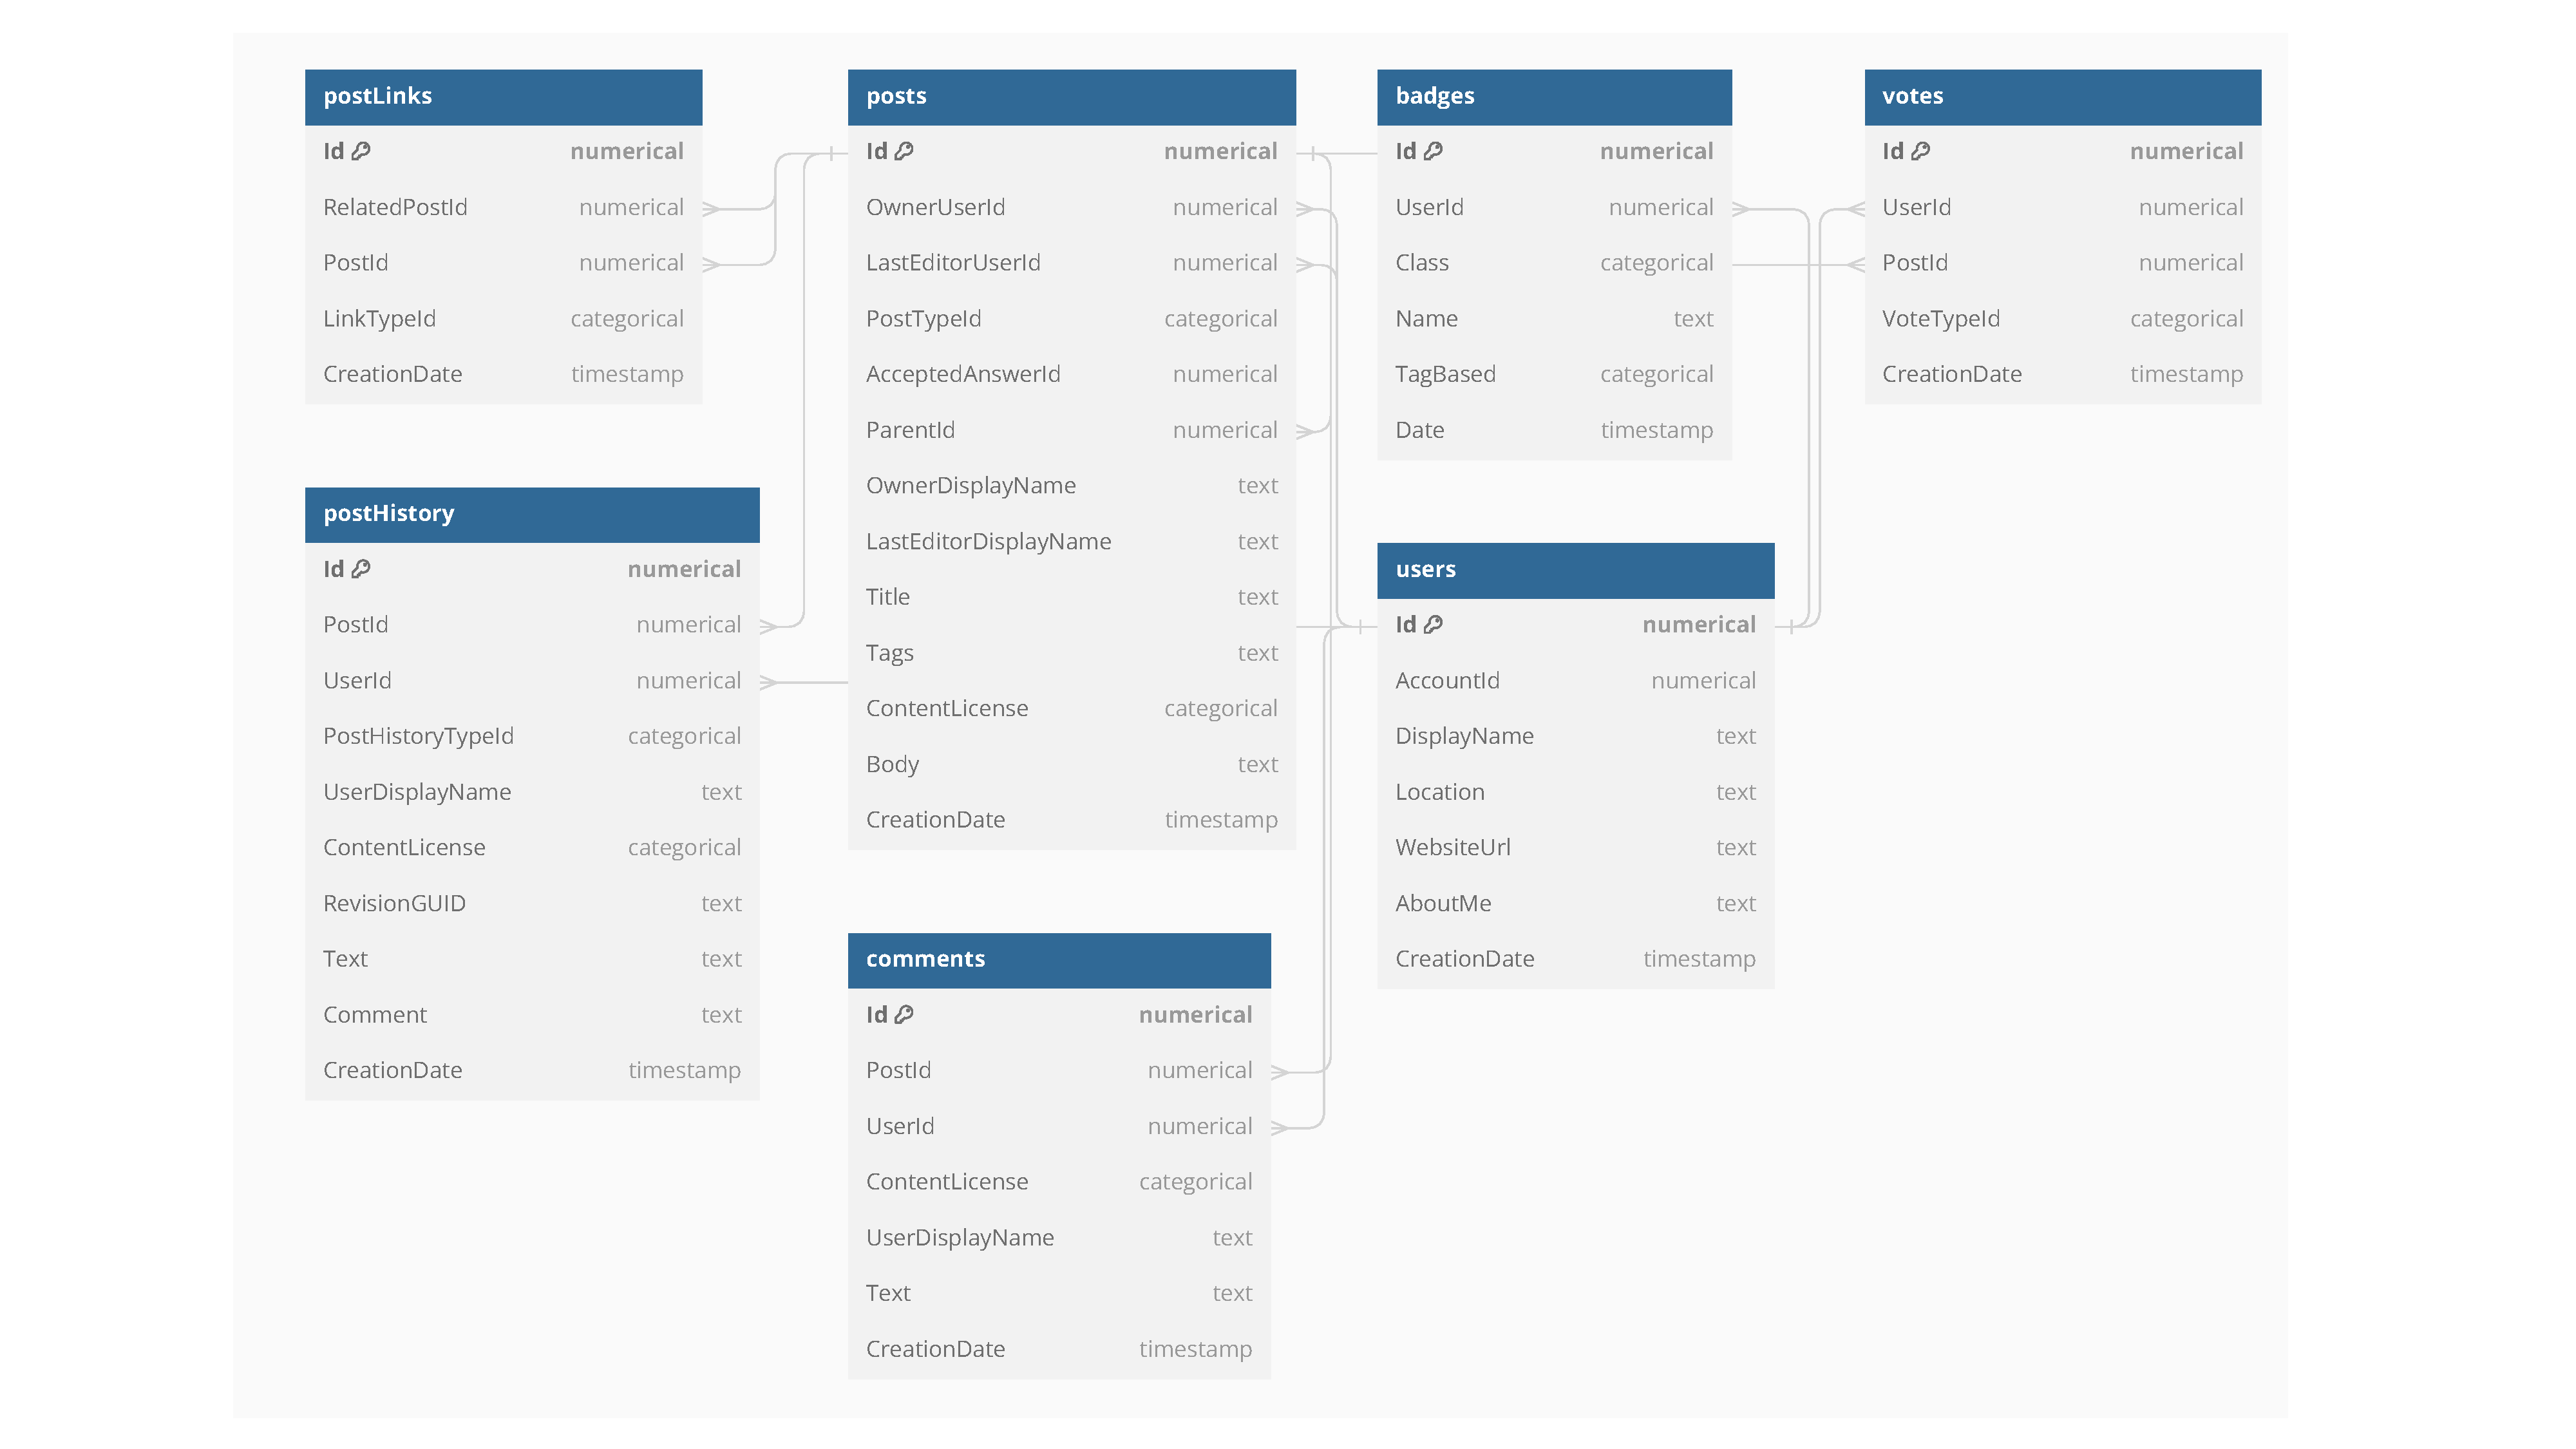
\includegraphics[width=\linewidth]{figs/stack-exchange.pdf}
  \caption{Entity relational diagrams of \texttt{Stack-Exchange}.}
  \label{fig:stack_exchange}
\end{figure}

\xhdr{Database overview} Stack Exchange is a network of question-and-answer websites on topics in diverse fields, each site covering a specific topic, where questions, answers, and users are subject to a reputation award process. The reputation system allows the sites to be self-moderating. In our benchmark, we use the stats-exchange site. We derive from the raw data dump from 2023-09-12. Figure~\ref{fig:stack_exchange} shows its entity relational diagrams. 

\xhdr{Dataset statistics} \StackEx covers 7 relational tables and contains 333K users, 415K posts, 794K comments, 1.67M votes, 103K post links, 590K badges records, 1.49M post history records. This relational database spans from 2009-02-02 to 2023-09-03. The validation timestamp $t_{\text{val}}$ is set to be 2019-01-01 and the testing timestamp $t_{\text{test}}$ is set to be 2021-01-01. Thus, the maximum time window size for predictive task is 2 years. 

\subsubsection{\StackExEngage: Predict if a user will be an active contributor to the site} 

\textbf{Task definition:} Predict if the user will make any contribution, defined as vote, comment, or post, to the site in the next 2 years. 

\textbf{Entity filtering:} We filter on active users defined as users that have made at least one comment/post/vote before the timestamp. 

\textbf{Task significance:} By accurately forecasting the levels of user contribution, website administrators can effectively gauge and oversee user activity. This insight allows for well-informed choices across various business aspects. For instance, it aids in preempting and mitigating user attrition, as well as in enhancing strategies to foster increased user interaction and involvement. This predictive task serves as a crucial tool in optimizing user experience and sustaining a dynamic and engaged user base.

\textbf{Machine learning task:} Binary classification. The label is 1 when user contributes to the site and 0 otherwise. 


\textbf{Evaluation metric:} Average Precision (AP).

\subsubsection{\StackExVotes: Predict the number of upvotes a question will receive}

\textbf{Task definition:} Predict the popularity of a question post in the next six months. The popularity is defined as the number of upvotes the post will receive.

\textbf{Entity filtering:} We filter on question posts that are posted recently in the past 2 years before the timestamp. This ensures that we do not predict on old questions that have been outdated.

\textbf{Task significance:} Predicting the popularity of a question post is valuable as it empowers site managers to predict and prepare for the influx of traffic directed towards that particular post. This foresight is instrumental in making strategic business decisions, such as curating question recommendations and optimizing content visibility. Understanding which posts are likely to attract more attention helps in tailoring the user experience and managing resources effectively, ensuring that the most engaging and relevant content is highlighted to maintain and enhance user engagement.

\textbf{Machine learning task:} Regression. The target ranges from 0-52 number of upvotes in the given time window in the training table.


\textbf{Evaluation metric:} Mean Absolute Error (MAE).




